\chapter{Introduction}
\label{intro}

\section{General Introduction}
This project concerns the development of a web application using a web framework in conjunction with a number of other tools. Throughout development, there is a particular cognisance towards the support of Non-Functional Requirements [NFRs] by both the web framework and the supporting tools throughout the development process. This project consists of both a software engineering component, in the shape of the web application developed using the tools discussed within this report, and a research component consisting of this report.

\section{Technology}

\begin{figure}[H]
\begin{center}
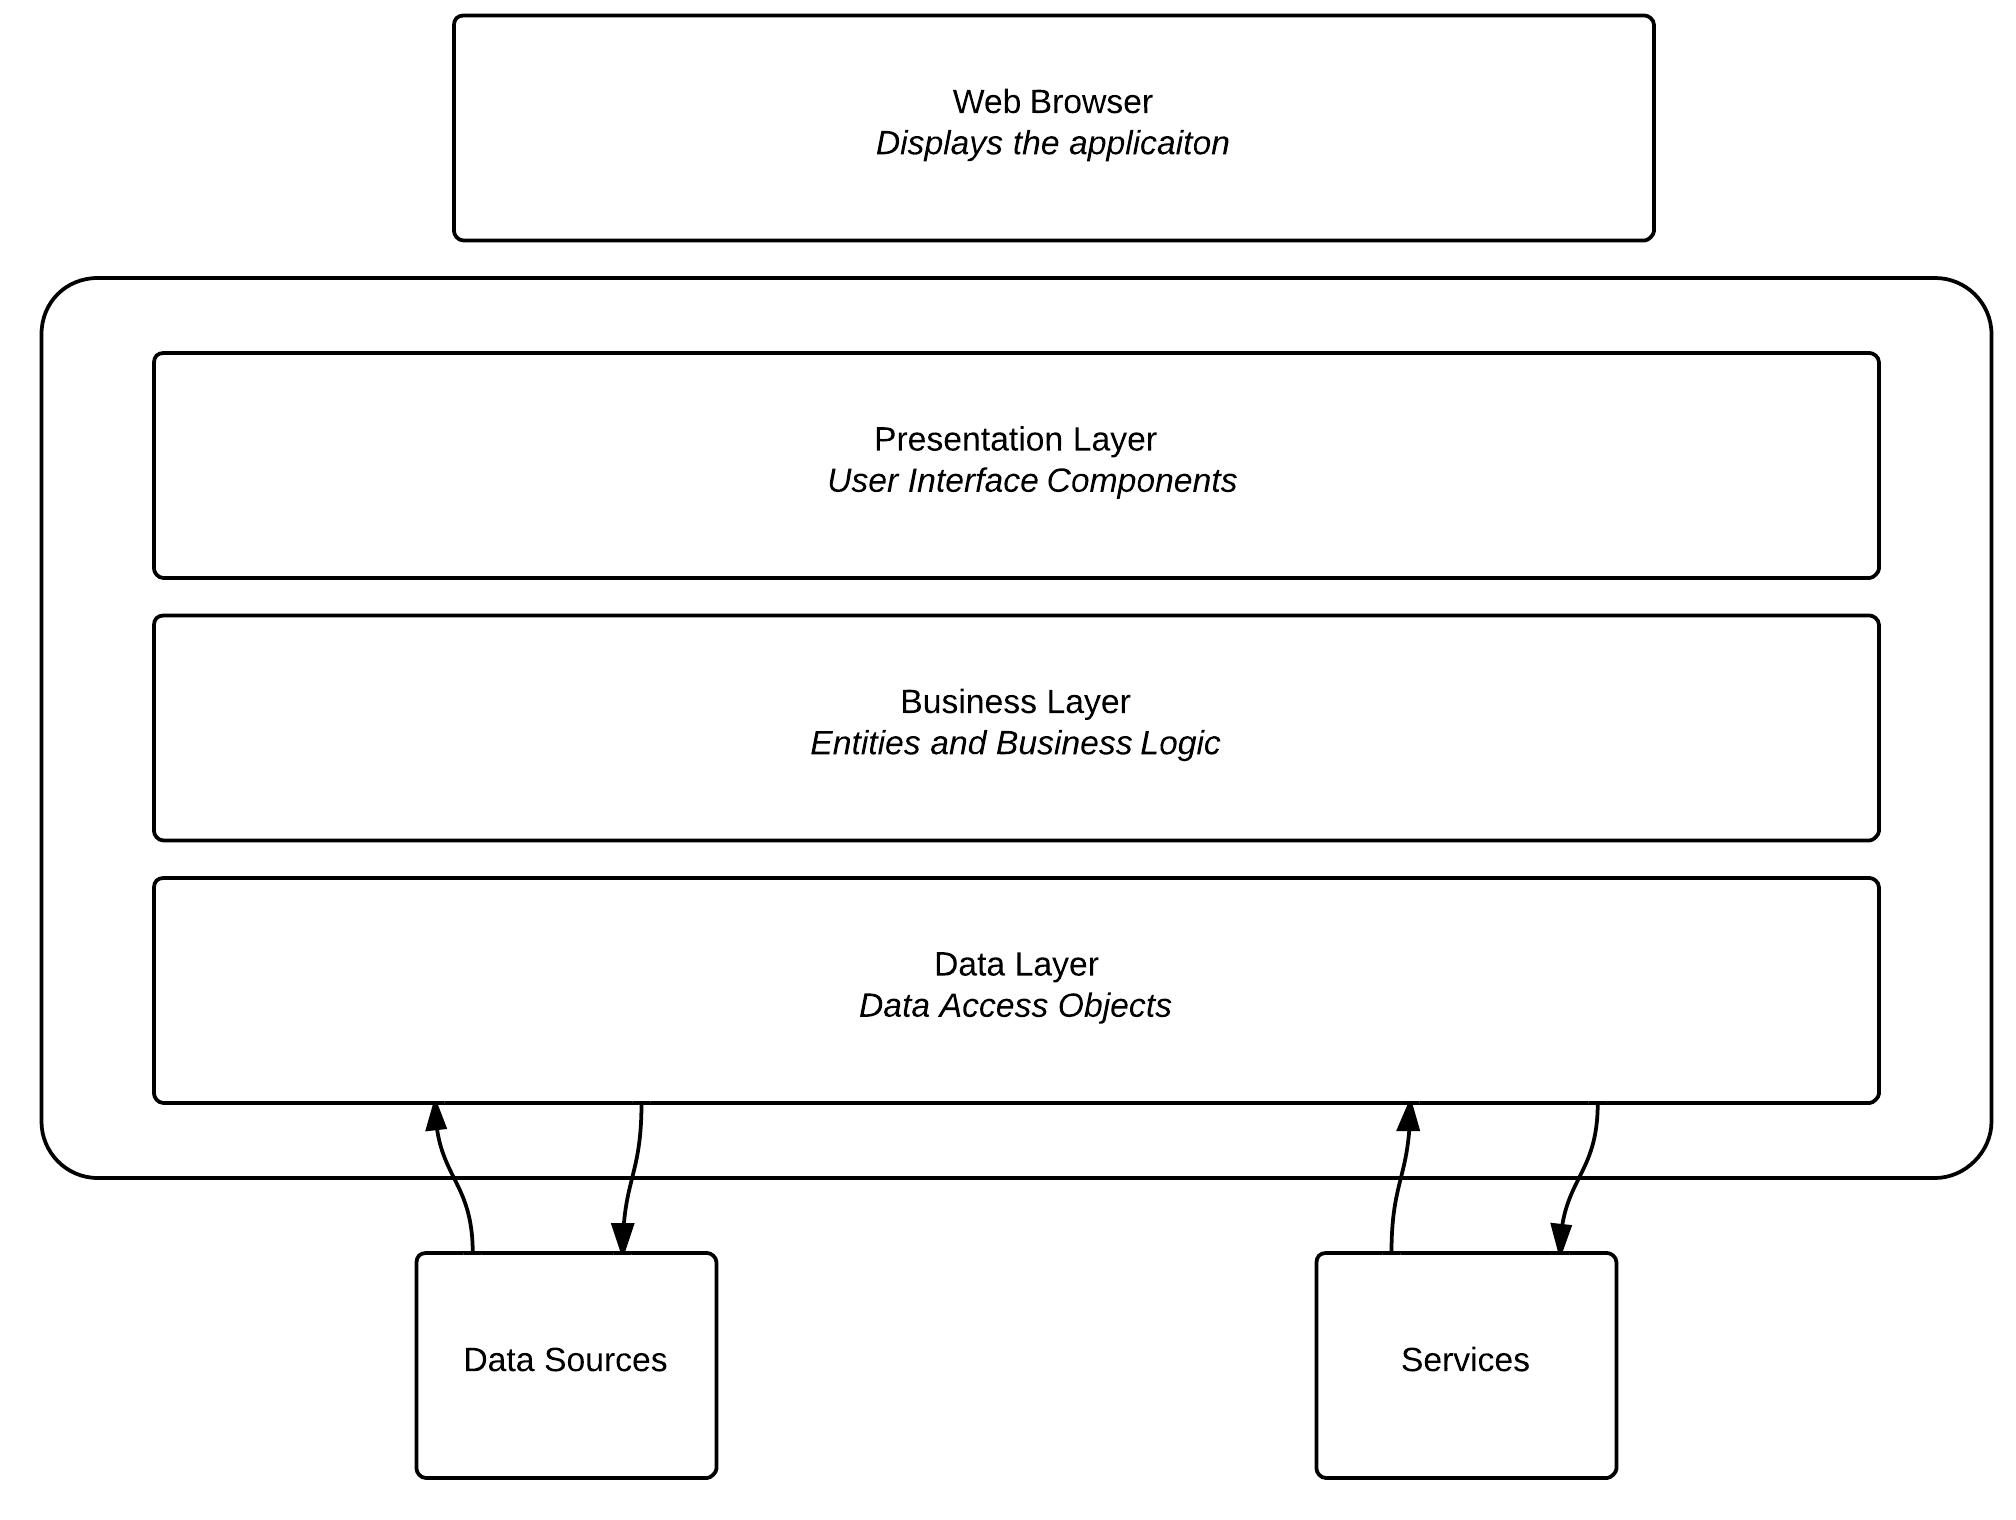
\includegraphics[scale=0.24]{webapp.PNG}
\end{center}
\caption{Typical architecture of a web application}
\end{figure}

\begin{figure}[H]
\begin{center}
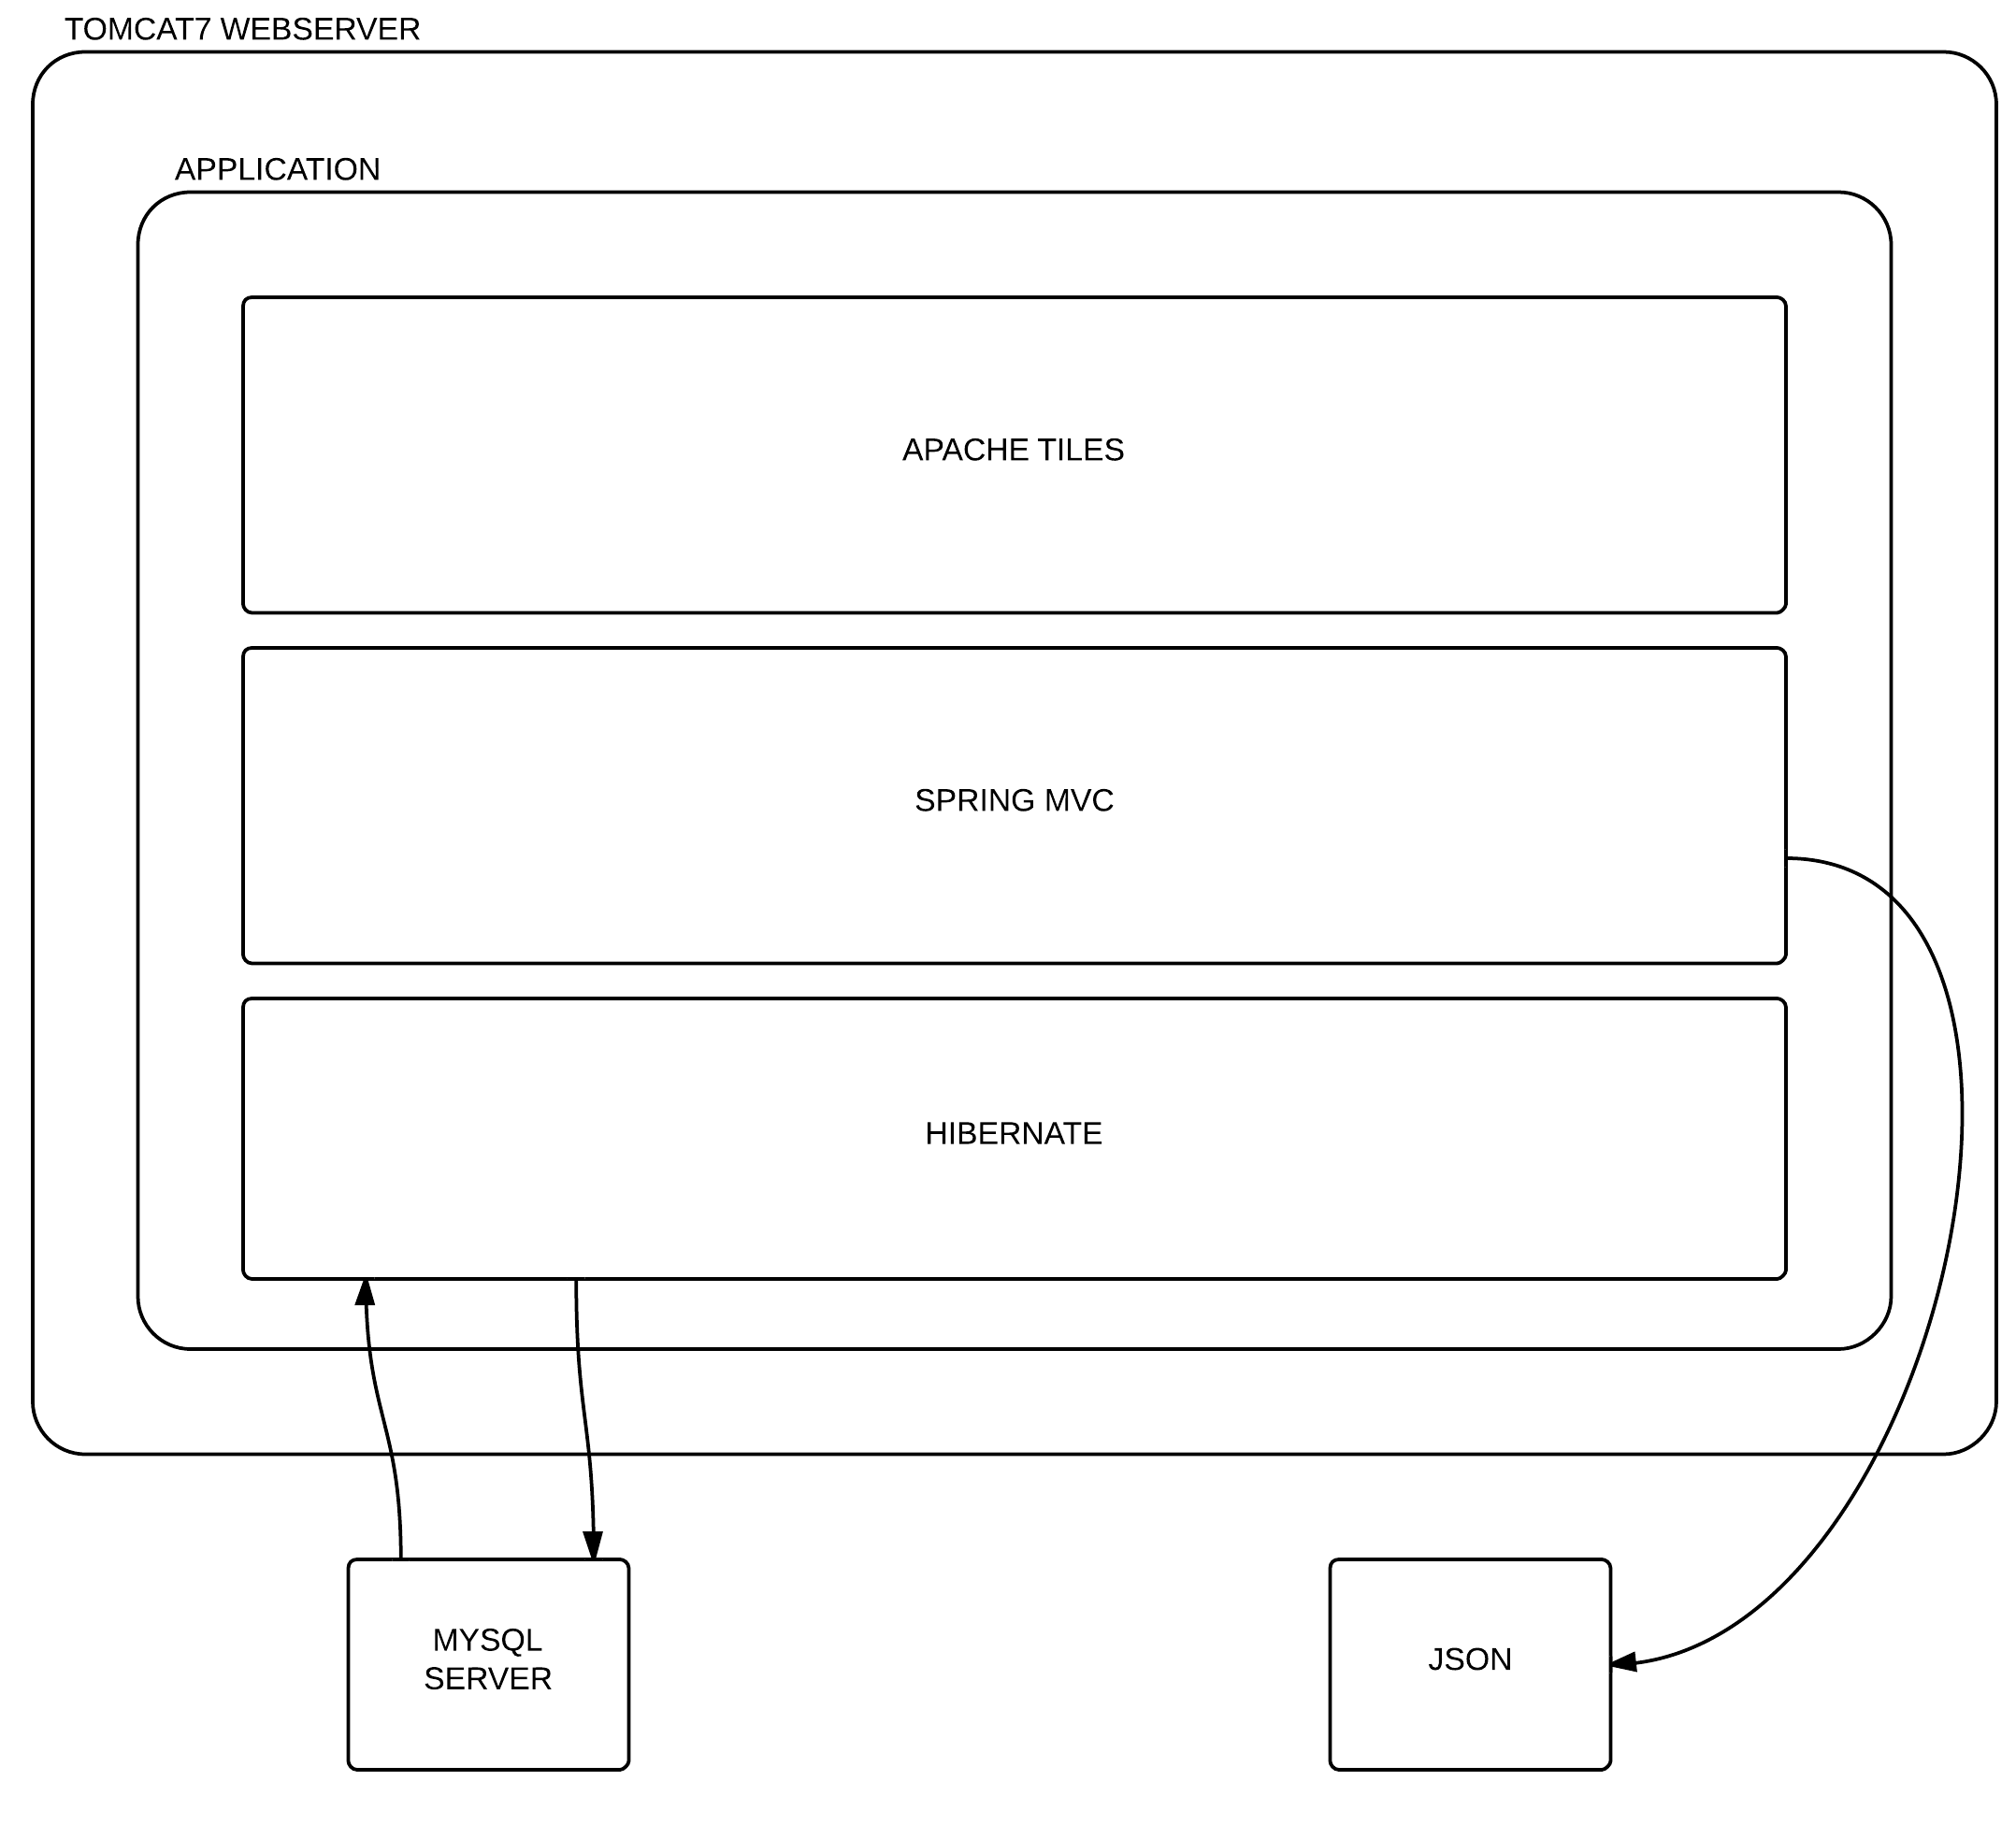
\includegraphics[scale=0.24]{projarch.PNG}
\end{center}
\caption{Typical architecture of a web application}
\end{figure}

\section{Objectives}

\subsection{Primary Objectives}

The primary objectives of this project are the support for quality attributes that the use of an architectural stack provides. The architectural stack within this project contains Spring MVC, Hibernate ORM and Apache Tiles. 

This project will examine the support provided for specific quality attributes: Security, Productivity, Extensibility and Performance. The provision of these attributed as provided by these frameworks will be examined, with cognisance of usability. 

\subsection{Secondary Objectives}

The secondary objectives of this project are: 

\begin{itemize}
\item To gain knowledge of the development of a web application using frameworks
\item To obtain experience working with a architectural stack common to industry
\item To use metrics and code visualisations within a project in order to guide and aid development of an application.
\end{itemize}

\section{Scope}



\section{Methodology}

The methodology used for this project was as follows

\begin{enumerate}
\item Learn the technology
\begin{itemize}
\item The first thing that was examined was the configuration of the technologies needed to implement a web application using Spring, Hibernate and Tiles. As such a set of tutorial videos provided by an educational website called Udemy provided a starting point. The paid videos totalled about 28 hours of content spread over 170 videos.\parencite{udemy}
\end{itemize}
\item Define objectives
\begin{itemize}
\item The next step was to define learning objectives from the project. The decision was made to focus on the support of specific quality attributes by the use of web application frameworks. This is the main objective of the paper, with secondary objectives relating to the use of metrics within a development in order to support overall quality of the application.
\end{itemize}
\item Requirements Engineering
\begin{itemize}
\item The elicitation of requirements from key stakeholders was an important step, and ensured that development of the application was in line with the expectations of those eventually utilising the application.
\end{itemize}
\item Design
\begin{itemize}
\item The design of the system, such as the structure for user authentication, and the overall design of the application were examined, with cognisance of design patterns.
\end{itemize}
\item Implementation, Testing and Deployment
\begin{itemize}
\item Once design of the application was completed, it needed to be implemented. Due to time constraints within a final year project, unit testing and some light user testing were the only techniques available to use. Deployment was a personal goal, as previous project had all been local applications.
\end{itemize}
\item Evaluation
\begin{itemize}
\item Evaluation of the application was performed by comparing the final application to methods use to other applications to achieve the same results. A usability study was also performed.
\end{itemize}
\end{enumerate}